\section{Results}

\subsection{Comparing Aggregate Statistics of Community Structure}

We begin by examining the overall statistics for the communities inferred by OSLOM using the weightings defined in Sections \ref{method-activity}, \ref{method-interaction}, and \ref{method-topic}. The number of communities by community type is given in Table~\ref{Table-comm_count}. We see that the topic- and interaction-based networks admit the most communities. The activity-based network admits the least number of communities.  One advantage of the OSLOM over many other community detection algorithms is that it explicitly accounts for singleton `communities': those nodes who do not belong to \emph{any} extant communities. This is especially important when a network is collected via a breadth-first search, as in our network, where we begin from a seed node and then branch out. Such a search, once terminated, will result in a collection of nodes on the periphery of the network that may not belong to any community in the core.

% See here
% 	http://arxiv.org/pdf/1202.2684v2.pdf
% for possible useful references on core-periphery networks.

The number of singletons by community type is also shown in Table~\ref{Table-comm_count}. We see that the topic- and interaction-based communities have the most singletons, with the activity-based community dominating this measure. This result for the activity-based community is an artifact of a property of the retweet/mention weighting: many of the users in the data set (\textbf{TK: give actual number}) did not interact with each other, and thus all of their edges were zero-weighted, leading to trivial singletons.

\begin{table}[ht]
	\label{Table-comm_count}
	\caption{Number of non-singleton communities and singletons by community type: S(tructural), A(ctivity -based), T(opic-based), and I(nteraction-based).}
	\centering
	\begin{tabular}{| c | c | c |}
		\hline Community Type & \# of Communities & \# of Singletons \\ \hline
		% Structural & 201 \\
		% Activity, Lag 1 & 101 \\
		% Activity, Lag 2 & 99 \\
		% Activity, Lag 3 & 106 \\
		% Activity, Lag 4 & 105 \\
		% Activity, Lag 5 & 107 \\
		% Activity, Lag 6 & 106 \\
		% Topic & 289 \\
		% Interaction & 252 \\ \hline
		S & 201 & 308 \\
		A, Lag 1 & 101 & 951 \\
		A, Lag 2 & 99 & 600 \\
		A, Lag 3 & 106 & 611 \\
		A, Lag 4 & 105 & 668 \\
		A, Lag 5 & 107 & 632 \\
		A, Lag 6 & 106 & 642 \\
		T & 289 & 1064 \\
		I & 252 & 2436 \\ \hline
	\end{tabular}
\end{table}

Next we consider the distribution of community sizes across the community types. The complementary cumulative distribution of community sizes is given in Figure~\ref{Fig-community_size_distribution}. Note that the axes are plotted on log-scale, and the horizontal axis begins with non-singleton communities. Thus, for a fixed community size $c$, Figure~\ref{Fig-community_size_distribution} shows the proportion of communities of size greater than $c$ for each community type. The largest communities for the structural, activity-based, topic-based, and interaction-based networks are 198, 358, 338, and 811 respectively.

\begin{figure}[ht]
  \centering
\includegraphics[width=0.50\textwidth]{Figures/comm_sizes_ecdf_loglog.pdf}
\caption{The proportion of communities greater than $c$ in size, across the different community types. Note the logarithmic scale on the horizontal and vertical axes.}
\label{Fig-community_size_distribution}
\end{figure}

Next, we compare the number of users which belong to more than one community. Figure~\ref{Fig-overlap_plot} shows the number of users belonging to 2, 3, or 4 communities. We see that as the number of mixed membership communities increases, the number of users with that number of mixed memberships decreases. This is especially true for the activity-based community \textbf{TK: speculate on what this means? Or save for the results section?}.  In addition, \textbf{TK: mention the 5, 6, and 7 cases, not included in the figure}. This corresponded to \textbf{TK: investigate which users are the high-overlap and what communities they belong to.}

% The user with a structural overlap of 7 communities was 1630261,
%	https://twitter.com/marksilva

\begin{figure}[ht]
  \centering
\includegraphics[width=0.50\textwidth]{Figures/overlap_by_type.pdf}
\caption{The number of users belonging to 2, 3, or 4 communities, by community type.}
\label{Fig-overlap_plot}
\end{figure}

\subsection{Comparing Community Types with Normalized Mutual Information}

Because OSLOM detects \emph{coverings} rather than \emph{partitions} of users, standard cluster comparison methods like variation of information~\cite{meilua2003comparing} are not appropriate. Instead, we use a generalization of variation of information measure first introduced in~\cite{lancichinetti2009detecting}, the normalized information. \textbf{TK: Etc. Put more here about NMI, what it does, and how to interpret it.}

The normalized mutual information between the various community-types are shown in Figure~\ref{Fig-compare_coverings}. We see that similarity between the coverings is dictated by the generic covering type, with distinct community structure between the structural, activity-based, and interaction-based communities. Interestingly, the communities resulting from the different weightings are all more similar to each other than to the structural communities from the unweighted network.Also note that the communities based on the hashtag similarities are different from both the activity-based and mention-retweet-based communities.

\begin{figure}[h!]
  \centering
\includegraphics[width=0.50\textwidth]{figures/nmi_singletons.pdf}
\caption{The normalized mutual information between the communities using the different weightings. Weighting 0 corresponds to the structural (binary weighting) network, weightings 1 through 6 correspond to the weighting using the transfer entropy with lag 1 through 6, weighting 7 corresponds to the hashtag similarity, and weightings 8, 9, and 10 correspond to the mention, retweet, and mention-retweet weightings. Values of normalized mutual information close to 1 indicate similarity in the community structure, while values close to 0 indicate dissimilarity. The normalized mutual information is computed with the singletons removed.}
\label{Fig-compare_coverings}
\end{figure}

\subsection{Comparing Edges Across Different Community-Types}

We have defined communities using four different criteria: structure, activity, interaction, and content. For a fixed community type, edges for a particular community may be partitioned into three sets: those from a node in the community to another node in the community (internal-to-internal), those from a node in the community to a node outside of the community (internal-to-external), and those from a node outside the community to a node inside the community (external-to-internal). See Figure~\ref{Fig-edge_types} for a schematic of this edge partitioning. For a meaningful community, we expect the distribution of weights within the community (internal-to-internal weights) to be different from the distribution of weights without the community (internal-to-external and external-to-internal).

\begin{figure}[h!]
  \centering
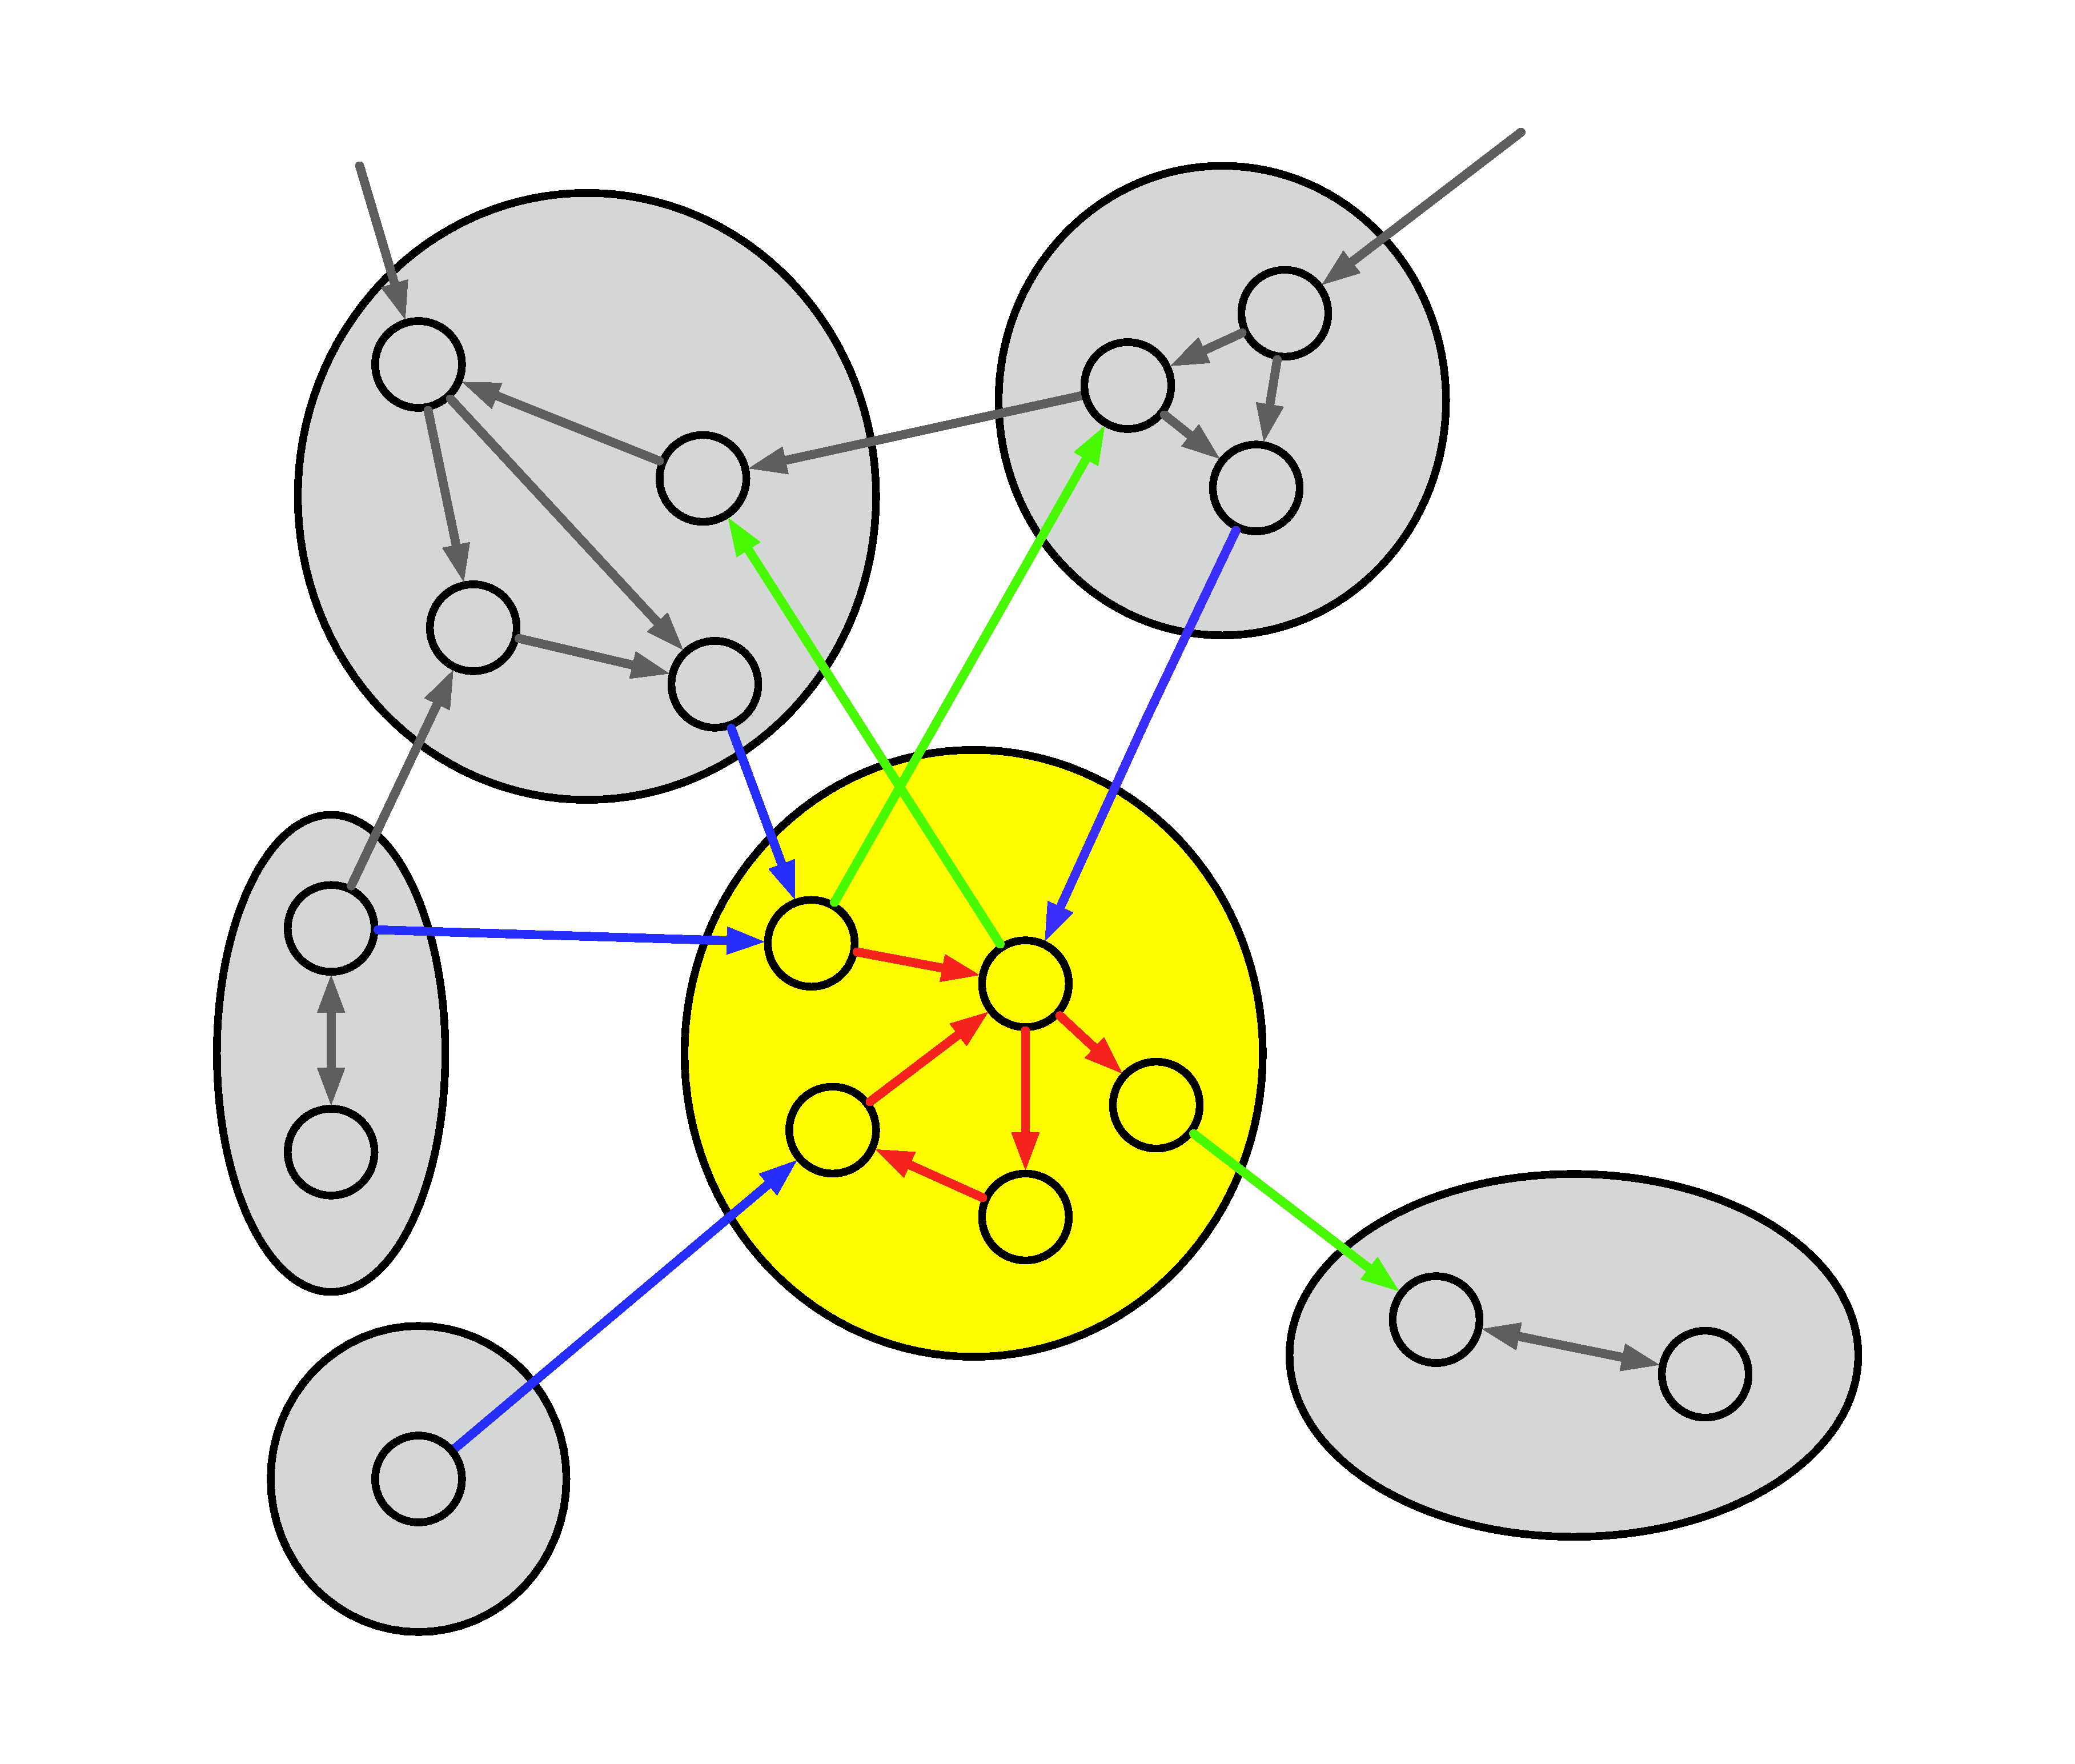
\includegraphics[width=0.50\textwidth]{figures/edge-types.eps}
\caption{An example of the edges considered in determining the edge weight distribution for a given community (the focal community is in yellow). We focus on the internal-to-internal (red), internal-to-external (green), and external-to-internal (blue) edges. For a given focal community, all other edges (grey) are not considered.}
\label{Fig-edge_types}
\end{figure}

For example, Figure~\ref{Fig-edge_types} shows the distributions of hashtag-based weights for the largest community defined by the mention-retweet network. We see that the distribution of internal-to-internal hashtag weights has a longer tail than either the external-to-internal or internal-to-external hashtag weights, with edges within the community having higher weights than edges crossing the boundary of the community. Thus, while the community was defined in terms of interactions, we still see a shift in the distribution of \emph{topic-similarity}.

\begin{figure}[h!]
  \centering
\includegraphics[width=0.50\textwidth]{Figures/comm0_labels-mention-retweet_weights-hashtag-ecdf.pdf}
\caption{The proportion of edges with a weight at least as large as the weight on the horizontal axis, across the types of edges described in Figure~\ref{Fig-edge_types}. The community is defined by user interactions, and the edge weights are determined by topics.}
\label{Fig-dist_across_community}
\end{figure}

This shift in the distribution was typical of many of the community type / weight pairings. To explore this further, for each of the top 100 largest communities defined by a particular community type (structure-based, behavior-based, content-based, or activity-based), we computed the median internal-to-internal, external-to-internal, and internal-to-external weight for that community for each weight type. These values summarize the typical value of each of these types of edges. We can then compute the ratio of the median internal-to-internal weight and the median external/internal-to-internal/external weight, which captures the proportional shift in the distribution. Finally, we compute the median of this proportional shift across all 100 of the largest communities. These values are summarized in Table~\ref{Table-medians}.

% \begin{table}
% 	\caption{The median value for the ratio of the median external/internal-to-internal/external weight to median internal-to-internal weight for the different community/weight pairings.}
% 	\centering
% 	\begin{tabular}{c | c | c  c  c  c}
% 		& & \multicolumn{4}{ c }{Community} \\ \hline
% 		\multirow{4}{*}{Weight} & & S & TE & MR & HT \\ \hline
% 		& TE & $0.0 / 0.0$ & $0.0 / 0.0$ & $0.0 / 0.0$ & $0.0 / 0.0$\\
% 		& MR & $0.0 / 0.0$ & $0.0 / 0.0$ & $0.0 / 0.0$ & $0.0 / 0.0$\\
% 		& HT & $0.0 / 0.0$ & $0.0 / 0.0$ & $0.0 / 0.0$ & $0.0 / 0.0$
% 	\end{tabular}
% \end{table}

\begin{table}
	\label{Table-medians}
	\caption{The median value across the 100 largest communities for the ratio of the median internal-to-internal weight to median external/internal-to-internal/external weight for the different community/weight pairings. \\ * For mention-retweet weights, weight zero edges were excluded from the computation of the median.}
	\centering
	\begin{tabular}{c | c | c  c  c}
		& & \multicolumn{3}{ c }{Weight} \\ \hline
		\multirow{4}{*}{Community} & & TE & MR & HT \\ \hline
		& S & $0.96/0.94$& $1.7/2.1$*& $9.0/8.0$\\
		& TE & $1.0/0.96$& $1.5/2.4$*& $24/17$\\
		& MR & $0.83/0.86$& $3.2/4.4$& $10/8.5$\\
		& HT & $0.9/0.89$& $2.4/2.6$*& $28/26$
	\end{tabular}
\end{table}

We see that overall, the 